Find the equation of line 
\begin{enumerate}[label=\thesubsection.\arabic*, ref=\thesubsection.\theenumi]
	\item passing through the point $\vec{P} = (– 4,  3)$ with slope $\frac{1}{2}$.
\label{chapters/11/10/2/2}
\\
\solution
Since the normal vector 
\begin{align}
\vec{n}=\myvec{\frac{1}{2}\\ -1}\\
\end{align}
the desired equation \eqref{eq:geo-normal} is 
\begin{align}
\vec{n}^\top \brak{\vec{x}-\vec{P}}&= 0 \\
\implies \myvec{\frac{1}{2}&-1}{\vec{x}}&=-5
\end{align}
See 
		\figref{fig:chapters/11/10/2/2/Figure}.
\begin{figure}[h]
\centering
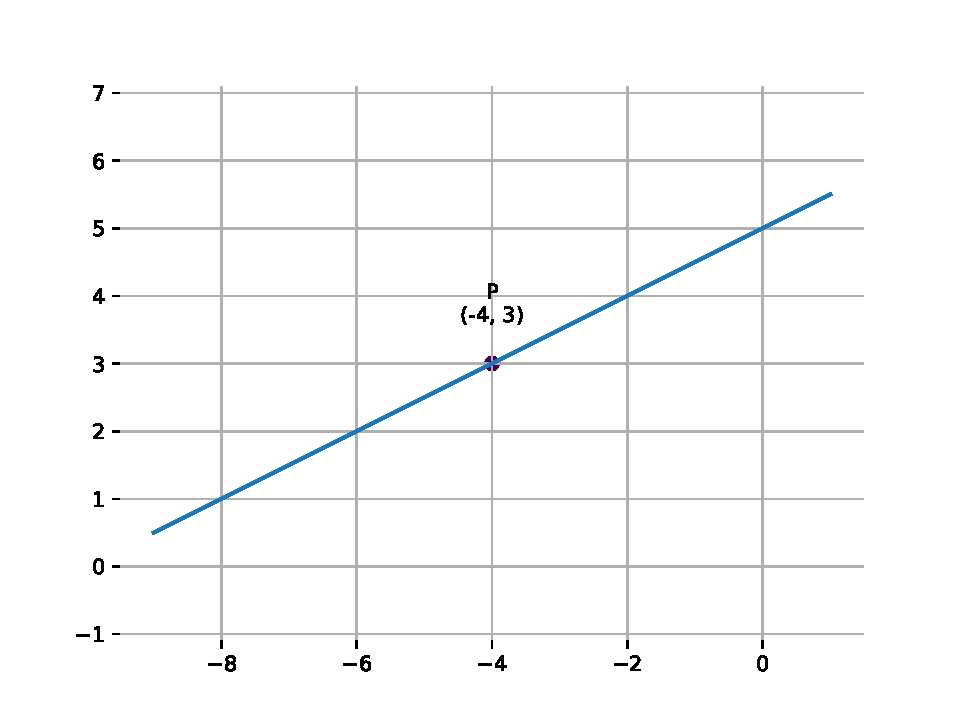
\includegraphics[width=\columnwidth]{chapters/11/10/2/2/figs/fig.pdf}
\caption{}
		\label{fig:chapters/11/10/2/2/Figure}
\end{figure}

	\item passing through $\myvec{0\\0}$ with slope $m$.\\
\label{chapters/11/10/2/3}
\solution
\iffalse
\documentclass[12pt]{article}
\usepackage{graphicx}
%\documentclass[journal,12pt,twocolumn]{IEEEtran}
\usepackage[none]{hyphenat}
\usepackage{graphicx}
\usepackage{listings}
\usepackage[english]{babel}
\usepackage{graphicx}
\usepackage{caption}
\usepackage[parfill]{parskip}
\usepackage{hyperref}
\usepackage{booktabs}
%\usepackage{setspace}\doublespacing\pagestyle{plain}
\def\inputGnumericTable{}
\usepackage{color}                                            %%
    \usepackage{array}                                            %%
    \usepackage{longtable}                                        %%
    \usepackage{calc}                                             %%
    \usepackage{multirow}                                         %%
    \usepackage{hhline}                                           %%
    \usepackage{ifthen}
\usepackage{array}
\usepackage{amsmath}   % for having text in math mode
\usepackage{parallel,enumitem}
\usepackage{listings}
\lstset{
language=tex,
frame=single, 
breaklines=true
}
  
%Following 2 lines were added to remove the blank page at the beginning
\usepackage{atbegshi}% http://ctan.org/pkg/atbegshi
\AtBeginDocument{\AtBeginShipoutNext{\AtBeginShipoutDiscard}}
%
%New macro definitions
\newcommand{\mydet}[1]{\ensuremath{\begin{vmatrix}#1\end{vmatrix}}}
\providecommand{\brak}[1]{\ensuremath{\left(#1\right)}}
\providecommand{\norm}[1]{\left\lVert#1\right\rVert}
\newcommand{\solution}{\noindent \textbf{Solution: }}
\newcommand{\myvec}[1]{\ensuremath{\begin{pmatrix}#1\end{pmatrix}}}
\let\vec\mathbf
\begin{document}
\begin{center}
\title{\textbf{Straight Lines}}
\date{\vspace{-5ex}} %Not to print date automatically
\maketitle
\end{center}
\setcounter{page}{1}
\section*{11$^{th}$ Maths - Chapter 10}
This is Problem-3 from Exercise 10.2
\begin{enumerate}
		\fi
		Line passing through point $\vec{A}=\myvec{0\\0}$ is given by,
\begin{align}
	\vec{n}^\top \brak{\vec{x}-\vec{A}} &= 0\label{eq:11/10/2/31}
\end{align}
Where,
		\begin{align}
			\vec{n} =\myvec{m \\ -1}
		\end{align}
		Substituting $\vec{A}$ and $\vec{n}$ in equation \eqref{eq:11/10/2/31}
		\begin{align}
			\myvec{m & -1}\brak{\vec{x}-\myvec{0\\0}} &=0\\
\implies			\myvec{m & -1}\vec{x} &= 0
		\end{align}
Line segment passing through $\myvec{0\\0}$ with slope $m = 2$ is shown in Fig. \ref{fig:11/10/2/3Fig1}
\begin{figure}[!h]
\begin{center}
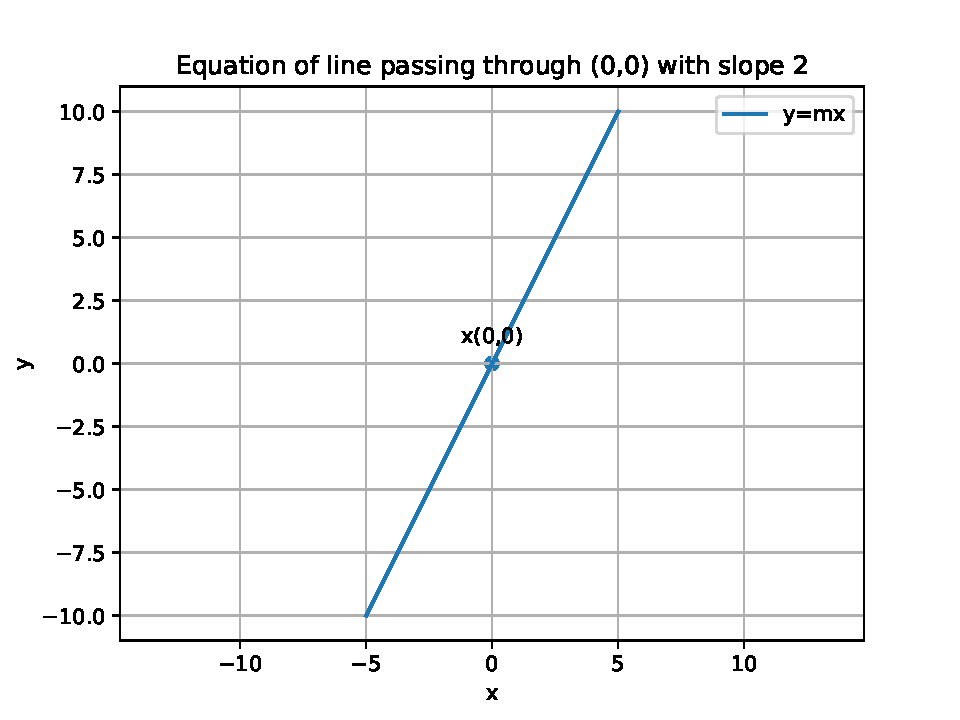
\includegraphics[width=\columnwidth]{chapters/11/10/2/3/figs/fig.pdf}
\end{center}
\caption{}
\label{fig:11/10/2/3Fig1}
\end{figure}

    \item passing through 
    $\vec{A} = \myvec{2\\2\sqrt{3}}$ and inclined with the x-axis at an angle 
    of 75\textdegree.
\label{chapters/11/10/2/4}
\\
    \solution 
    \begin{align}
	    \vec{n} &= \myvec{-1\\2+\sqrt{3}}
        \label{eq:11/10/2/4normal-vec}
	\\
	    \implies
        \implies \vec{n}^\top\vec{x} = \vec{n}^\top\vec{A} &= 4\brak{\sqrt{3}+1} \\
        \implies \myvec{-1&2+\sqrt{3}}\vec{x} &=\myvec{-1&2+\sqrt{3}}\myvec{2\\2\sqrt{3}}  
	    \\
	    &= 4\brak{\sqrt{3}+1}
        \label{eq:11/10/2/4line}
    \end{align}
is the desired equation.  See \figref{fig:11/10/2/4line}.
    \begin{figure}[!ht]
        \centering
        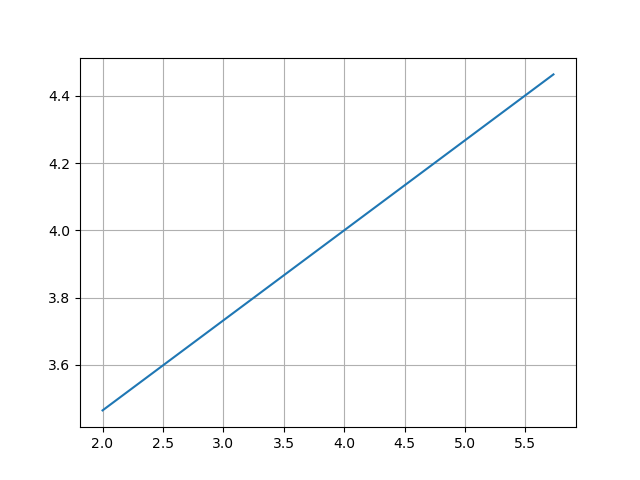
\includegraphics[width=\columnwidth]{chapters/11/10/2/4/figs/line.png}
        \caption{}
        \label{fig:11/10/2/4line}
    \end{figure}

\item intersecting the x-axis at a distance of 3 units to the left of origin with slope of -2.
\label{chapters/11/10/2/5}
\\
\solution 
		From the given information,
\begin{align}		
	\vec{A}=\myvec{-3\\0},\,
\vec{n} = \myvec{2 \\1}.
\end{align}
The desired equation of the line is
\begin{align}
\implies	\myvec { 2 & 1 } \brak{ \vec{x} - \myvec{ -3 \\ 0}} &= 0  \\
	\text{or, }	\myvec{ 2 & 1} \vec{x}  &= -6
        \label{eq:chapters/11/10/2/5/1}
\end{align}
See \figref{fig:chapters/11/10/2/5/Fig1}.
\begin{figure}[H]
	\begin{center}
		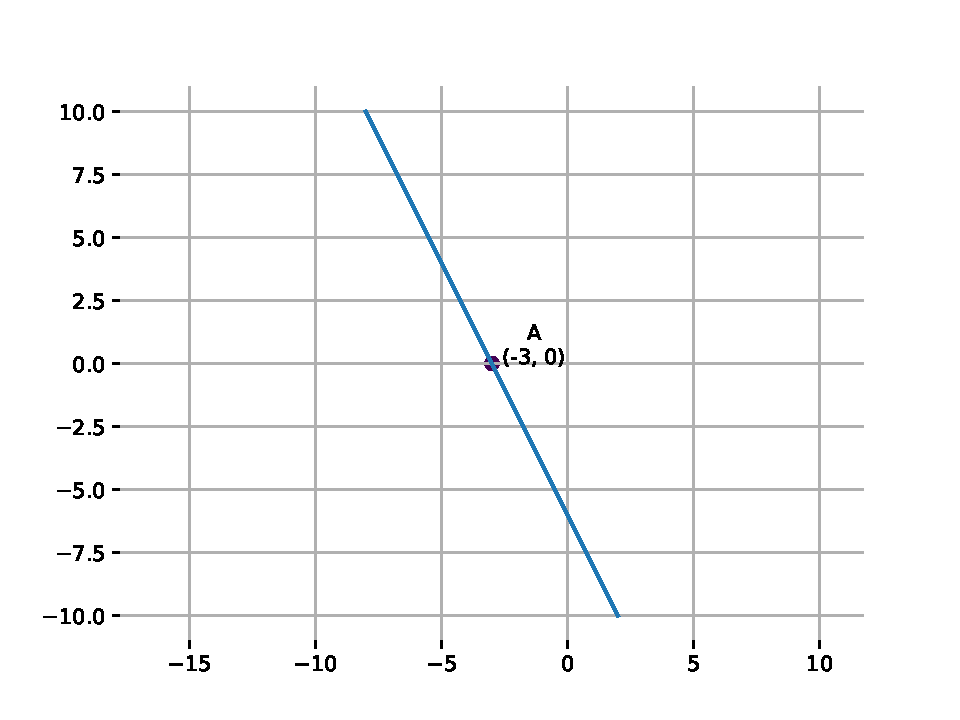
\includegraphics[width=0.75\columnwidth]{chapters/11/10/2/5/figs/fig.pdf}
	\end{center}
\caption{}
\label{fig:chapters/11/10/2/5/Fig1}
\end{figure}


\item intersecting the y-axis at a distance of 2 units above the origin and making an
angle of $30\degree$ with positive direction of the x-axis.
\\
\solution 
\iffalse
\documentclass[journal,12pt,twocolumn]{IEEEtran}
\usepackage{setspace}
\usepackage{gensymb}
\usepackage{xcolor}
\usepackage{caption}
\singlespacing
\usepackage{siunitx}
\usepackage[cmex10]{amsmath}
\usepackage{mathtools}
\usepackage{hyperref}
\usepackage{amsthm}
\usepackage{mathrsfs}
\usepackage{txfonts}
\usepackage{stfloats}
\usepackage{cite}
\usepackage{cases}
\usepackage{subfig}
\usepackage{longtable}
\usepackage{multirow}
\usepackage{enumitem}
\usepackage{bm}
\usepackage{mathtools}
\usepackage{listings}
\usepackage{tikz}
\usetikzlibrary{shapes,arrows,positioning}
\usepackage{circuitikz}
\renewcommand{\vec}[1]{\boldsymbol{\mathbf{#1}}}
\DeclareMathOperator*{\Res}{Res}
\renewcommand\thesection{\arabic{section}}
\renewcommand\thesubsection{\thesection.\arabic{subsection}}
\renewcommand\thesubsubsection{\thesubsection.\arabic{subsubsection}}

\renewcommand\thesectiondis{\arabic{section}}
\renewcommand\thesubsectiondis{\thesectiondis.\arabic{subsection}}
\renewcommand\thesubsubsectiondis{\thesubsectiondis.\arabic{subsubsection}}
\hyphenation{op-tical net-works semi-conduc-tor}

\lstset{
language=Python,
frame=single, 
breaklines=true,
columns=fullflexible
}
\begin{document}
\theoremstyle{definition}
\newtheorem{theorem}{Theorem}[section]
\newtheorem{problem}{Problem}
\newtheorem{proposition}{Proposition}[section]
\newtheorem{lemma}{Lemma}[section]
\newtheorem{corollary}[theorem]{Corollary}
\newtheorem{example}{Example}[section]
\newtheorem{definition}{Definition}[section]
\newcommand{\BEQA}{\begin{eqnarray}}
        \newcommand{\EEQA}{\end{eqnarray}}
\newcommand{\define}{\stackrel{\triangle}{=}}
\newcommand{\myvec}[1]{\ensuremath{\begin{pmatrix}#1\end{pmatrix}}}
\newcommand{\mydet}[1]{\ensuremath{\begin{vmatrix}#1\end{vmatrix}}}
\bibliographystyle{IEEEtran}
\providecommand{\nCr}[2]{\,^{#1}C_{#2}} % nCr
\providecommand{\nPr}[2]{\,^{#1}P_{#2}} % nPr
\providecommand{\mbf}{\mathbf}
\providecommand{\pr}[1]{\ensuremath{\Pr\left(#1\right)}}
\providecommand{\qfunc}[1]{\ensuremath{Q\left(#1\right)}}
\providecommand{\sbrak}[1]{\ensuremath{{}\left[#1\right]}}
\providecommand{\lsbrak}[1]{\ensuremath{{}\left[#1\right.}}
\providecommand{\rsbrak}[1]{\ensuremath{{}\left.#1\right]}}
\providecommand{\brak}[1]{\ensuremath{\left(#1\right)}}
\providecommand{\lbrak}[1]{\ensuremath{\left(#1\right.}}
\providecommand{\rbrak}[1]{\ensuremath{\left.#1\right)}}
\providecommand{\cbrak}[1]{\ensuremath{\left\{#1\right\}}}
\providecommand{\lcbrak}[1]{\ensuremath{\left\{#1\right.}}
\providecommand{\rcbrak}[1]{\ensuremath{\left.#1\right\}}}
\theoremstyle{remark}
\newtheorem{rem}{Remark}
\newcommand{\sgn}{\mathop{\mathrm{sgn}}}
\newcommand{\rect}{\mathop{\mathrm{rect}}}
\newcommand{\sinc}{\mathop{\mathrm{sinc}}}
\providecommand{\abs}[1]{\left\vert#1\right\vert}
\providecommand{\res}[1]{\Res\displaylimits_{#1}}
\providecommand{\norm}[1]{\lVert#1\rVert}
\providecommand{\mtx}[1]{\mathbf{#1}}
\providecommand{\mean}[1]{E\left[ #1 \right]}
\providecommand{\fourier}{\overset{\mathcal{F}}{ \rightleftharpoons}}
\providecommand{\ztrans}{\overset{\mathcal{Z}}{ \rightleftharpoons}}
\providecommand{\system}[1]{\overset{\mathcal{#1}}{ \longleftrightarrow}}
\newcommand{\solution}{\noindent \textbf{Solution: }}
\providecommand{\dec}[2]{\ensuremath{\overset{#1}{\underset{#2}{\gtrless}}}}
\let\StandardTheFigure\thefigure
\def\putbox#1#2#3{\makebox[0in][l]{\makebox[#1][l]{}\raisebox{\baselineskip}[0in][0in]{\raisebox{#2}[0in][0in]{#3}}}}
\def\rightbox#1{\makebox[0in][r]{#1}}
\def\centbox#1{\makebox[0in]{#1}}
\def\topbox#1{\raisebox{-\baselineskip}[0in][0in]{#1}}
\def\midbox#1{\raisebox{-0.5\baselineskip}[0in][0in]{#1}}

\vspace{3cm}
\title{11.10.2.6}
\author{Lokesh Surana}
\maketitle
\section*{Class 11, Chapter 10, Exercise 2.6}


\solution 
\fi
The direction vector of the line is given by
\begin{align}
    \vec{m} = \myvec{1 \\ \tan(30\degree)} = \myvec{1 \\ \frac{1}{\sqrt{3}}}
\end{align}
The normal vector $\vec{n}$ to the line is given by
\begin{align}
    \vec{n} =  \myvec{-\frac{1}{\sqrt{3}} \\ 1}
\end{align}
The line is passing through the point 
\begin{align}
    \vec{A} = \myvec{0 \\ 2}
\end{align}
Hence, 
the equation of the line is given by
\begin{align}
    \vec{n}^\top\brak{\vec{x}-\vec{A}} &= 0 \\
    \implies \myvec{-\frac{1}{\sqrt{3}}&1}\brak{ \vec{x} - \myvec{0 \\ 2}} &= 0  \\
    \text{or, }	\myvec{-\frac{1}{\sqrt{3}}&1} \vec{x}  &= 2
\end{align}
%
\begin{figure}[!htb]
    \centering
    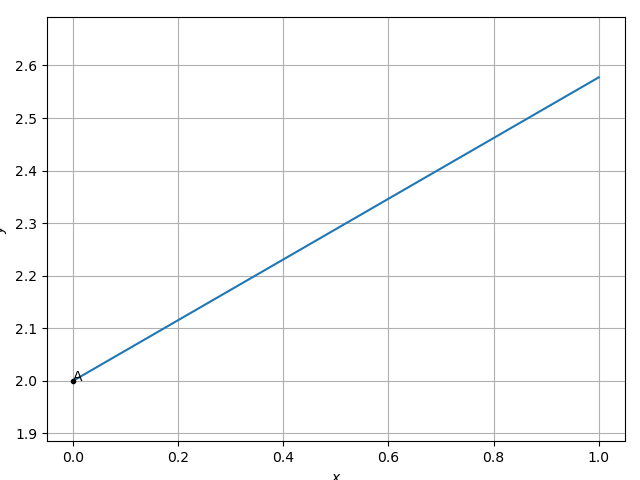
\includegraphics[width=\columnwidth]{chapters/11/10/2/6/figs/line.png}
    \caption{}
    \label{fig:chapters/11/10/2/6/line}
\end{figure}


\item passing through (1, 2) and making angle $30\degree$ with $y$-axis.
\item passing through the points $\vec{A}\myvec{-1\\1}$ and $\vec{B}\myvec{2\\-4}$.
\label{chapters/11/10/2/7}
\\
\solution 
\begin{align}
	\vec{m} &= \vec{A} - \vec{B}
= \myvec{-3\\5}
\implies
\vec{n} &= \myvec{5\\3}
\end{align}
Thus, the equation of line is
\begin{align}
 \myvec{ 5 & 3}\vec{x}  &= -2
\end{align}
See 
   \figref{fig:chapters/11/10/2/7/Line_AB}.
\begin{figure}[h!]
  \centering
   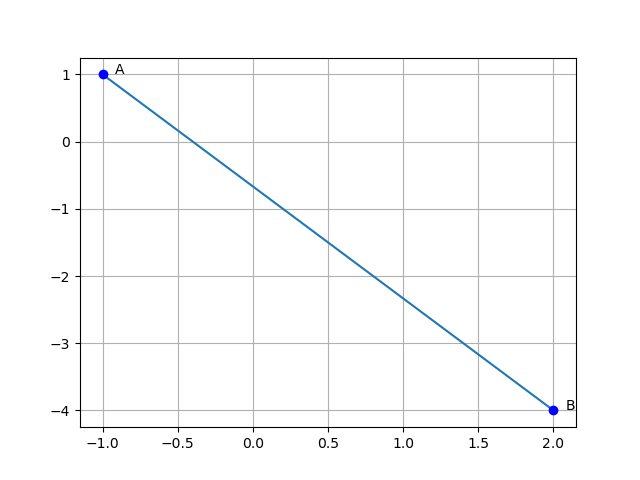
\includegraphics[width=\linewidth]{chapters/11/10/2/7/figs/Figure_1.png}
   \caption{}
   \label{fig:chapters/11/10/2/7/Line_AB}
\end{figure}





\item passing through the points $(3, 4, -7)$ and $(1, -1, 6)$. 
\item The vector equation of the line 
\begin{align*}
	\frac{x-5}{3}=\frac{y+4}{7}=\frac{z-6}{2} 
\end{align*}
is \noindent\rule{2cm}{0.4pt}. 
\item The vector equation of the line 
\begin{align*}
	\frac{x-5}{3}=\frac{y+4}{7}=\frac{z-6}{2}
\end{align*}
 is \noindent\rule{2cm}{0.4pt}.
\item 
The vertices of triangle $PQR$ are $\vec{P}(2, 1),  \vec{Q}(-2, 3),  \vec{R}(4, 5)$. Find the equation of the median through $\vec{R}$.
\label{chapters/11/10/2/9}
\\
\solution
	\begin{figure}[H]
		\centering
 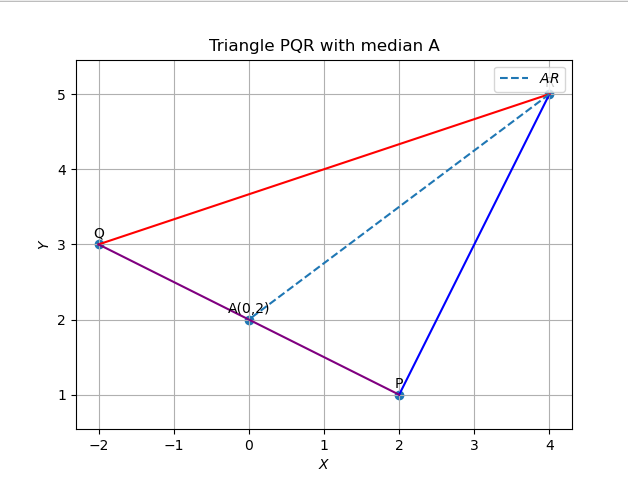
\includegraphics[width=0.75\columnwidth]{chapters/11/10/2/9/figs/line.png}
		\caption{}
		\label{fig:11/10/2/9}
  	\end{figure}
	See Fig. 
		\ref{fig:11/10/2/9}.
Using section formula, the mid point of $PQ$ is
\begin{align}
\vec{A} = \frac{\vec{P} +\vec{Q} }{2}
	= {\myvec{0\\2}}
\end{align} 
Following the approach in \probref{chapters/11/10/2/7},
\begin{align*}
	\augvec{2}{1}{ 
	4 & 5 & 1
	\\  
	0 & 2 & 1
	}
	\xleftrightarrow[R_2 \leftarrow 4R_2 ]{R_1 \leftarrow 2R_1 -5R_2}
	\augvec{2}{1}{ 
	8 & 0 & -3 
	\\ 
	0 & 8 & 4 
	}
	\implies \vec{n} = \frac{1}{8}\myvec{ -3 \\ 4}
\end{align*}
Thus,
the equation of the line is 
\begin{align}
	\myvec{-3 & 4}\vec{x} =8 
\end{align}

	\item Find the equations of the planes that pass through the points
\begin{enumerate}
\item $\vec{A}= \myvec{1\\1\\– 1},  \vec{B}=\myvec{6\\4\\– 5}, \vec{C}= \myvec{– 4\\– 2\\3}$
\item $\vec{A}= \myvec{1\\1\\0},  \vec{B}= \myvec{1\\2\\1},  \vec{C}= \myvec{– 2\\2\\-1}$
\end{enumerate}
    \solution
		\begin{enumerate}
	\item From 
		\eqref{prop:lin-eq-unit-mat},
\begin{align}
\myvec{1&1&-1\\ 6&4&-5\\ -4&-2&3} \vec{n} = \myvec{1\\1\\1}
\end{align}
\begin{align*}
	\implies \myvec{1&1&-1&\vrule&1\\6&4&-5&\vrule&1\\-4&-2&3&\vrule&1}
	\\
\xleftrightarrow[R_3 \leftarrow R_3 + 4R_1]{R_2 \leftarrow R_2 - 6R_1}
\myvec{1&1&-1&\vrule&1\\0&-2&1&\vrule&-5\\0&2&-1&\vrule&5}\\ 
\xleftrightarrow[{R_1 \leftarrow 2R_1 + R_2}] {R_3 \leftarrow R_3 + R_2}
\myvec{2&0&-1&\vrule&-3\\0&2&-1&\vrule&5\\0&0&0&\vrule&0}
\end{align*}
Since we obtain a 0 row, 
the given points are collinear.
The direction vector of the line is
\begin{align}
\vec{m}=\vec{B}-\vec{C} \equiv \myvec{5\\3\\-4}
\end{align}
and the equation of a line is given by,
\begin{align}
	\vec{x}&=\vec{A}+  \kappa\vec{m}\\
&= \myvec{1\\1\\– 1} + \kappa \myvec{5\\3\\-4}
\end{align}
See 
     \figref{fig:chapters/12/11/3/6/1}.
\begin{figure}[h!]
  \centering
   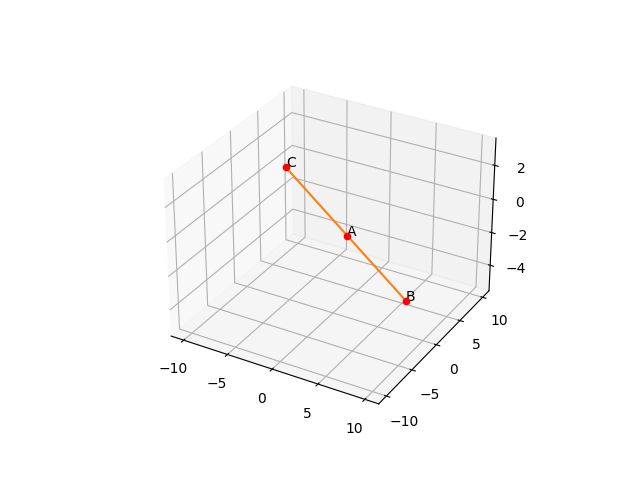
\includegraphics[width=\columnwidth]{chapters/12/11/3/6/figs/collinear_points.png}
    \caption{}
     \label{fig:chapters/12/11/3/6/1}
     \end{figure}
     \item  In this case, 
\begin{align}
\myvec{1&1&0 \\ 1&2&1 \\ -2&2&-1} \vec{n}=\vec{1}
\end{align}
\begin{align*}
\implies
\myvec{1&1&0&\vrule&1\\1&2&1&\vrule&1\\-2&2&-1&\vrule&1}
\\
\xleftrightarrow[R_3 \leftarrow R_3 + 2R_1]{R_2 \leftarrow R_2 - R_1}
\myvec{1&1&0&\vrule&1\\0&1&1&\vrule&0\\0&4&-1&\vrule&3}
\\
	\xleftrightarrow[R_3 \leftarrow R_3 - 4R_2]{R_1 \leftarrow R_1- R_2}
\myvec{1&0&-1&\vrule&1\\0&1&1&\vrule&0\\0&0&-5&\vrule&3}\\
	\xleftrightarrow[R_2 \leftarrow 5R_2 + R_3]{R_1 \leftarrow 5R_1- R_3}
\myvec{5&0&0&\vrule&2\\0&5&0&\vrule&3\\0&0&5&\vrule&-3}
\end{align*}
Hence, the equation of the plane is
\begin{align}
\myvec{2 & 3 & -3} \vec{x} = 5
\end{align}
\end{enumerate}

\item Find the equation of the plane through the points $(2, 1, 0)$,  $(3, -2, -2)$ and $(3, 1, 7)$.
\item A plane passes through the points $(2, 0, 0),  (0, 3, 0)$ and $(0, 0, 4)$. The equation of the plane is \noindent\rule{2cm}{0.4pt}.
\item If the intercept of a line between the coordinate axes is divided by the point (-5, 4) in the ratio 1:2 then find the equation of the line.
\item Find the equation of a line that cuts off equal intercepts on the coordinate axes and passes through the point $(2, 3)$.  
	\\
\solution 
\label{chapters/11/10/2/12}
Let $(a,0)$  and  $(0,a)$ be the intercept points. 
\begin{align}
\vec{m} 
        &=   \myvec{
		a \\
		0 
		} - \myvec{
		   0 \\
		   a
		}  
        		  \equiv \myvec{
                           1 \\
			   -1 
		         } 
			 \\
			 \implies
\vec{n} &=  \myvec{
		     1 \\
		     1
	     } 
\end{align}
and 
the equation of the  line is
\begin{align}
	\myvec { 1 & 1 } \brak{ \vec{ x  - \myvec{ 2 \\
                                   3
			     }
		}}  &= 0  \\
\implies		\myvec{ 1 & 1} \vec{x}  &= 5 
        \label{eq:11/10/2/12/1}
\end{align}
See  \figref{fig:11/10/2/12/Fig1}.
\begin{figure}[H]
	\begin{center}
		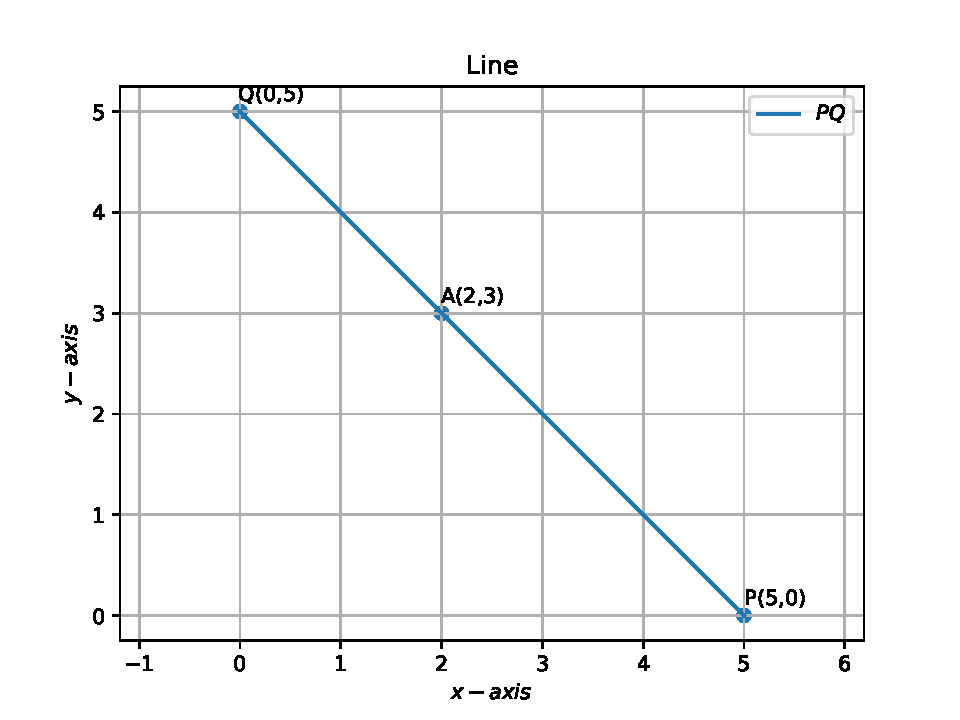
\includegraphics[width=0.75\columnwidth]{chapters/11/10/2/12/figs/problem12.pdf}
	\end{center}
\caption{}
\label{fig:11/10/2/12/Fig1}
\end{figure}


\item 
Find the equation of a line passing through a point (2, 2) and cutting off intercepts on the axes whose sum is 9.
\label{chapters/11/10/2/13}
	\\
	\solution 
Let  the intercept points be
\begin{align}
{\vec{P}}=\myvec{
  a\\
  0}
 , {\vec{Q}}=\myvec{
  0\\
  b}
  \text{ and }
   {\vec{R}}=\myvec{
  2\\
  2}
\end{align}
be the given point.  
Forming the collinearity matrix from 
		\eqref{prop:lin-dep-rank},
\begin{align}
	\myvec{ \vec{P}-\vec{Q} &\vec{P}-\vec{R}} 
	=
	 \myvec{
  a & a-2\\
  -b & -2
 }
\end{align}
which is singular if 
\begin{align}
 ab -2\brak{a+b} = 0
 \implies ab = 18
		\label{eq:11/10/2/13-a+b}
		\\
\because  a + b = 9.
\end{align}
$\therefore a,b$
are the roots of
\begin{align}
	x^2 -9x +18 = 0.
\end{align}
yielding
\begin{align}
	\myvec{a \\ b} = \myvec{6 \\ 3}, \myvec{3\\6}
\end{align}
Since 
\begin{align}
	\vec{m} = \myvec{a \\ -b},
	\vec{n} = \myvec{b \\ a} \equiv \myvec{1 \\ 2}, \myvec{2\\1}
\end{align}
Thus, the possible equations of the line are 
\begin{align}
\myvec{1 & 2}\vec{x} = 6
	\\
	\myvec{2&1}\vec{x} = 6
\end{align}
		See \figref{fig:11/10/2/13}.
	\begin{figure}[H]
		\centering
 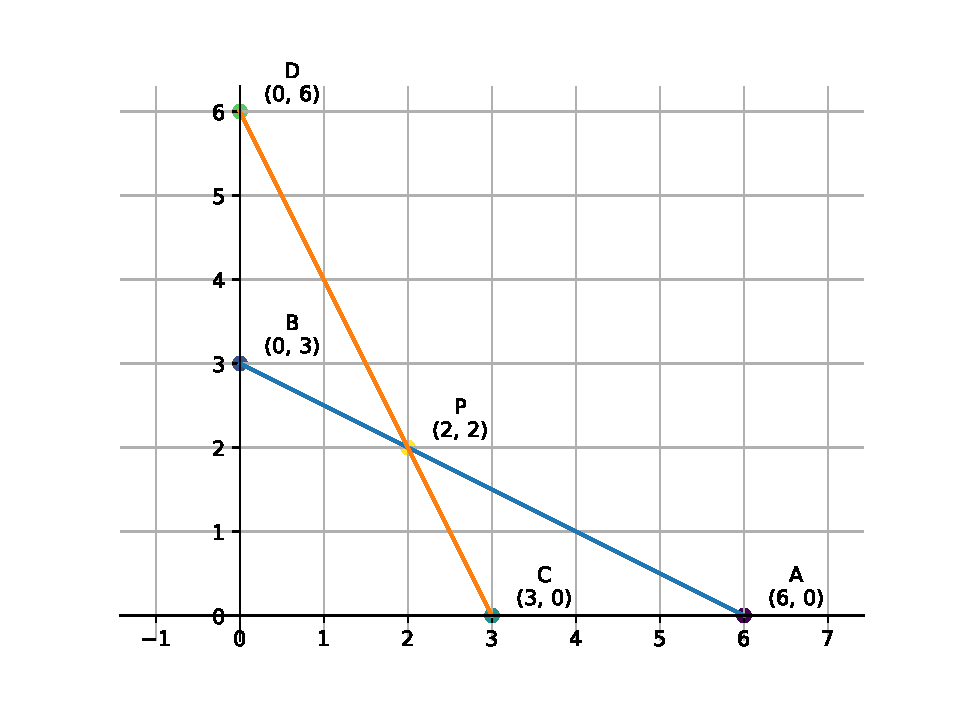
\includegraphics[width=0.75\columnwidth]{chapters/11/10/2/13/figs/fig.pdf}
		\caption{}
		\label{fig:11/10/2/13}
  	\end{figure}

\item Find the equation of the lines which passes the point (3, 4) and cuts off intercepts from the coordinate axes such that their sum is 14.
\item Find the equation of the straight line which passes through the point (1,  -2) and cuts off equal intercepts from axes.
\item Find the equation of the line which passes through the point (-4, 3) and the portion of the line intercepted between the axes is divided internally in ratio 5:3 by this point.
\item Consider the following population and year graph. Find the slope of the line AB and using it,  find what will be the population in the year 2010.
\\
\begin{figure}[H]
\centering
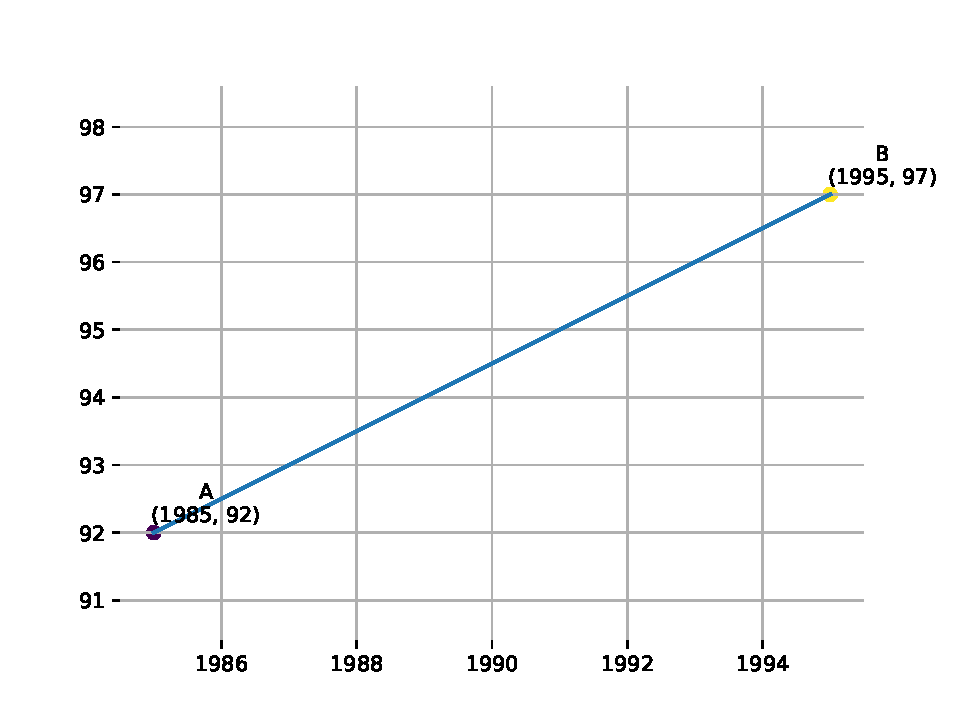
\includegraphics[width=0.75\columnwidth]{chapters/11/10/1/14/figs/fig.png}
\caption{}
\label{fig:chapters/11/10/1/14/1}
\end{figure}
\solution
The direction vector of the line in \figref{fig:chapters/11/10/1/14/1} is
\begin{align}
\vec{m} = \vec{B} - \vec{A}
= \myvec{2 \\ 1}
\\
\implies \vec{n}
= \myvec{1 \\ -2}
\end{align}
 The equation of the line is then given by 
\begin{align}
\vec{n}^{\top} (\vec{x} -\vec{A}) &= 0 \\
\implies 
\myvec{1& -2} \vec{x} &= 1801
\\
\implies  \myvec{1&-2} \myvec{2010\\y} &= 1801 \\
\implies y &= \frac{209}{2}
\end{align}





\item Slope of a line which cuts off intercepts of equal length on the axes is 
\begin{enumerate}
\item -1
\item -0
\item 2
\item $\sqrt{3}$
\end{enumerate}
\item If the coordinates of middle point of the portion of a line intercepted between the coordinate axes is (3, 2), then the equation of the line will be
\begin{enumerate}
\item $2x+3y=12$
\item $3x+2y=12$
\item $4x-3y=6$
\item $5x-2y=10$
\end{enumerate}
\item If the line $\frac{x}{a}+\frac{y}{b}=1$ passes the points (2, -3) and (4, -5),  then $(a, b)$ is 
\begin{enumerate}
\item (1, 1)
\item (-1, 1)
\item (1, -1)
\item (-1, -1)
\end{enumerate}
\item The intercepts made by the plane $2x-3y+5z+4=0$ on the co-ordinate axis are $\brak{-2, \frac{4}{3}, -\frac{4}{5}}$.
\item The line $\overrightarrow{r}=2\hat{i}-3\hat{j}-\hat{k}+\lambda(\hat{i}-\hat{j}+2\hat{k})$ lies in the plane $\overrightarrow{r} \cdot (3\hat{i}+\hat{j}-\hat{k})+2=0$.
\item Find the equation of the line joining $(1, 2)$ and $(3, 6)$.
\item Find the equation of the line joining $(3, 1)$ and $(9, 3)$.
\item If the point (3,  4) lies on the line $3y=ax+7$,  find the value of $a$.
\item  Find the equation of the line that passes through the point with position vector $2\hat{i}-\hat{j}+4\hat{k}$ and is in direction $\hat{i}+2\hat{j}-\hat{k}$.
\item The cartesian equation of a line is $ \frac{x-5}{3}=\frac{y+4}{7}=\frac{z-6}{2}$. Write its vector form.
\item Find the equation of the line that passes through the origin and $(5, -2, 3)$.
\item Find the equation of the line that passes through the points $(3, -2, -5), (3, -2, 6)$.
\item Find the coordinates of the point where the line through $(5,1,6)$ and $(3,4,1)$ crosses the $YZ$-plane.
\item Find the coordinates of the point where the line through $(5,1,6)$ and $(3,4,1)$ crosses the $ZX$-plane.
\item Find the coordinates of the point where the line through $(3,-4,-5)$ and $(2,-3,1)$ crosses the plane $2x+y+x=7$.
\item Find the equation of the line through $(-2,3)$ with slope $-4$
\item Write the equation of the line through the points $(1,-1)$ and $(3,5)$.
\item Write the equation of the lines for which $\tan \theta=\frac{1}{2}$, where $\theta$ is the inclination of the line and
\begin{enumerate}
\item  y-intercept is $\frac{-3}{2}$ 
\item  x-intercept is $4$.
\end{enumerate}
\item Find the equation of the lines which makes intercepts $-3$ and $2$ on the x- and y-axes respectively.
\item Equation of a line is $3x-4y+10=0$, Find its
\begin{enumerate}
\item  Slope
\item  x and y-intercepts.
\end{enumerate}
\item The Fahrenheit temperature $F$ and  absolute temperature $K$ satisfy a linear equation. Given that $K=273$ when $F=32$ and that $K=373$ when $F=212$. Express $K$ in terms of $F$ and find the value of $F$, when $K=0$.
\item A line is such that its segment between the lines $5x-y+4=0$ and $3x+4y-4=0$ is bisected at the point $(1,5)$. Obtain its equation.
\end{enumerate}
